\textbf{Thấu kính tứ cực từ hội tụ mạnh}

Trong các máy gia tốc hạt năng lượng cao, việc điều hướng chuyển động của các hạt cần thông qua các tương tác điện từ. Tứ cực từ là một mô hình từ trường tạo ra bởi hệ thống dây điện được cuốn để sinh ra từ trường có dạng đường sức khá giống với bốn nam châm đặt đối xứng bốn góc và thường được sử dụng cho mục đích điều hướng chùm hạt. Trường điện từ của tứ cực từ sẽ tác dụng lực lên các hạt khiến cho quỹ đạo của chúng bị bẻ cong như cách các tia sáng đi qua các thấu kính quang học, nhưng lại chỉ bẻ hướng tia sáng về phía quang trục (như thấu kính hội tụ) theo một phương và bẻ hướng tia sáng ra xa khỏi quang trục (như thấu kính phân kỳ) theo phương còn lại. Trong bài toán này, chúng ta sẽ khảo sát định tính về mô hình tứ cực từ cũng như thiết kế một hệ các thấu kính tứ cực để tạo ra sự hội tụ cho chùm hạt.


\begin{enumerate}
    \item \textbf{Tính chất thú vị của tứ cực từ} \\
    Khi bạn lắp ráp bốn nam châm điện lại thành một hệ sao cho hai cực Nam ở đối diện nhau và hai cực Bắc ở đối diện nhau như hình \ref{fig:41}, bạn sẽ thu được một \textbf{tứ cực từ}. Tứ cực từ có rất nhiều tính chất thú vị, và được sử dụng rộng rãi trong các máy gia tốc hạt nhằm hội tụ các chùm tia tích điện. Các câu hỏi phía dưới sẽ khảo sát các đặc tính độc đáo của tứ cực từ:
    
    \begin{center}
    \begin{minipage}{0.45\textwidth}
    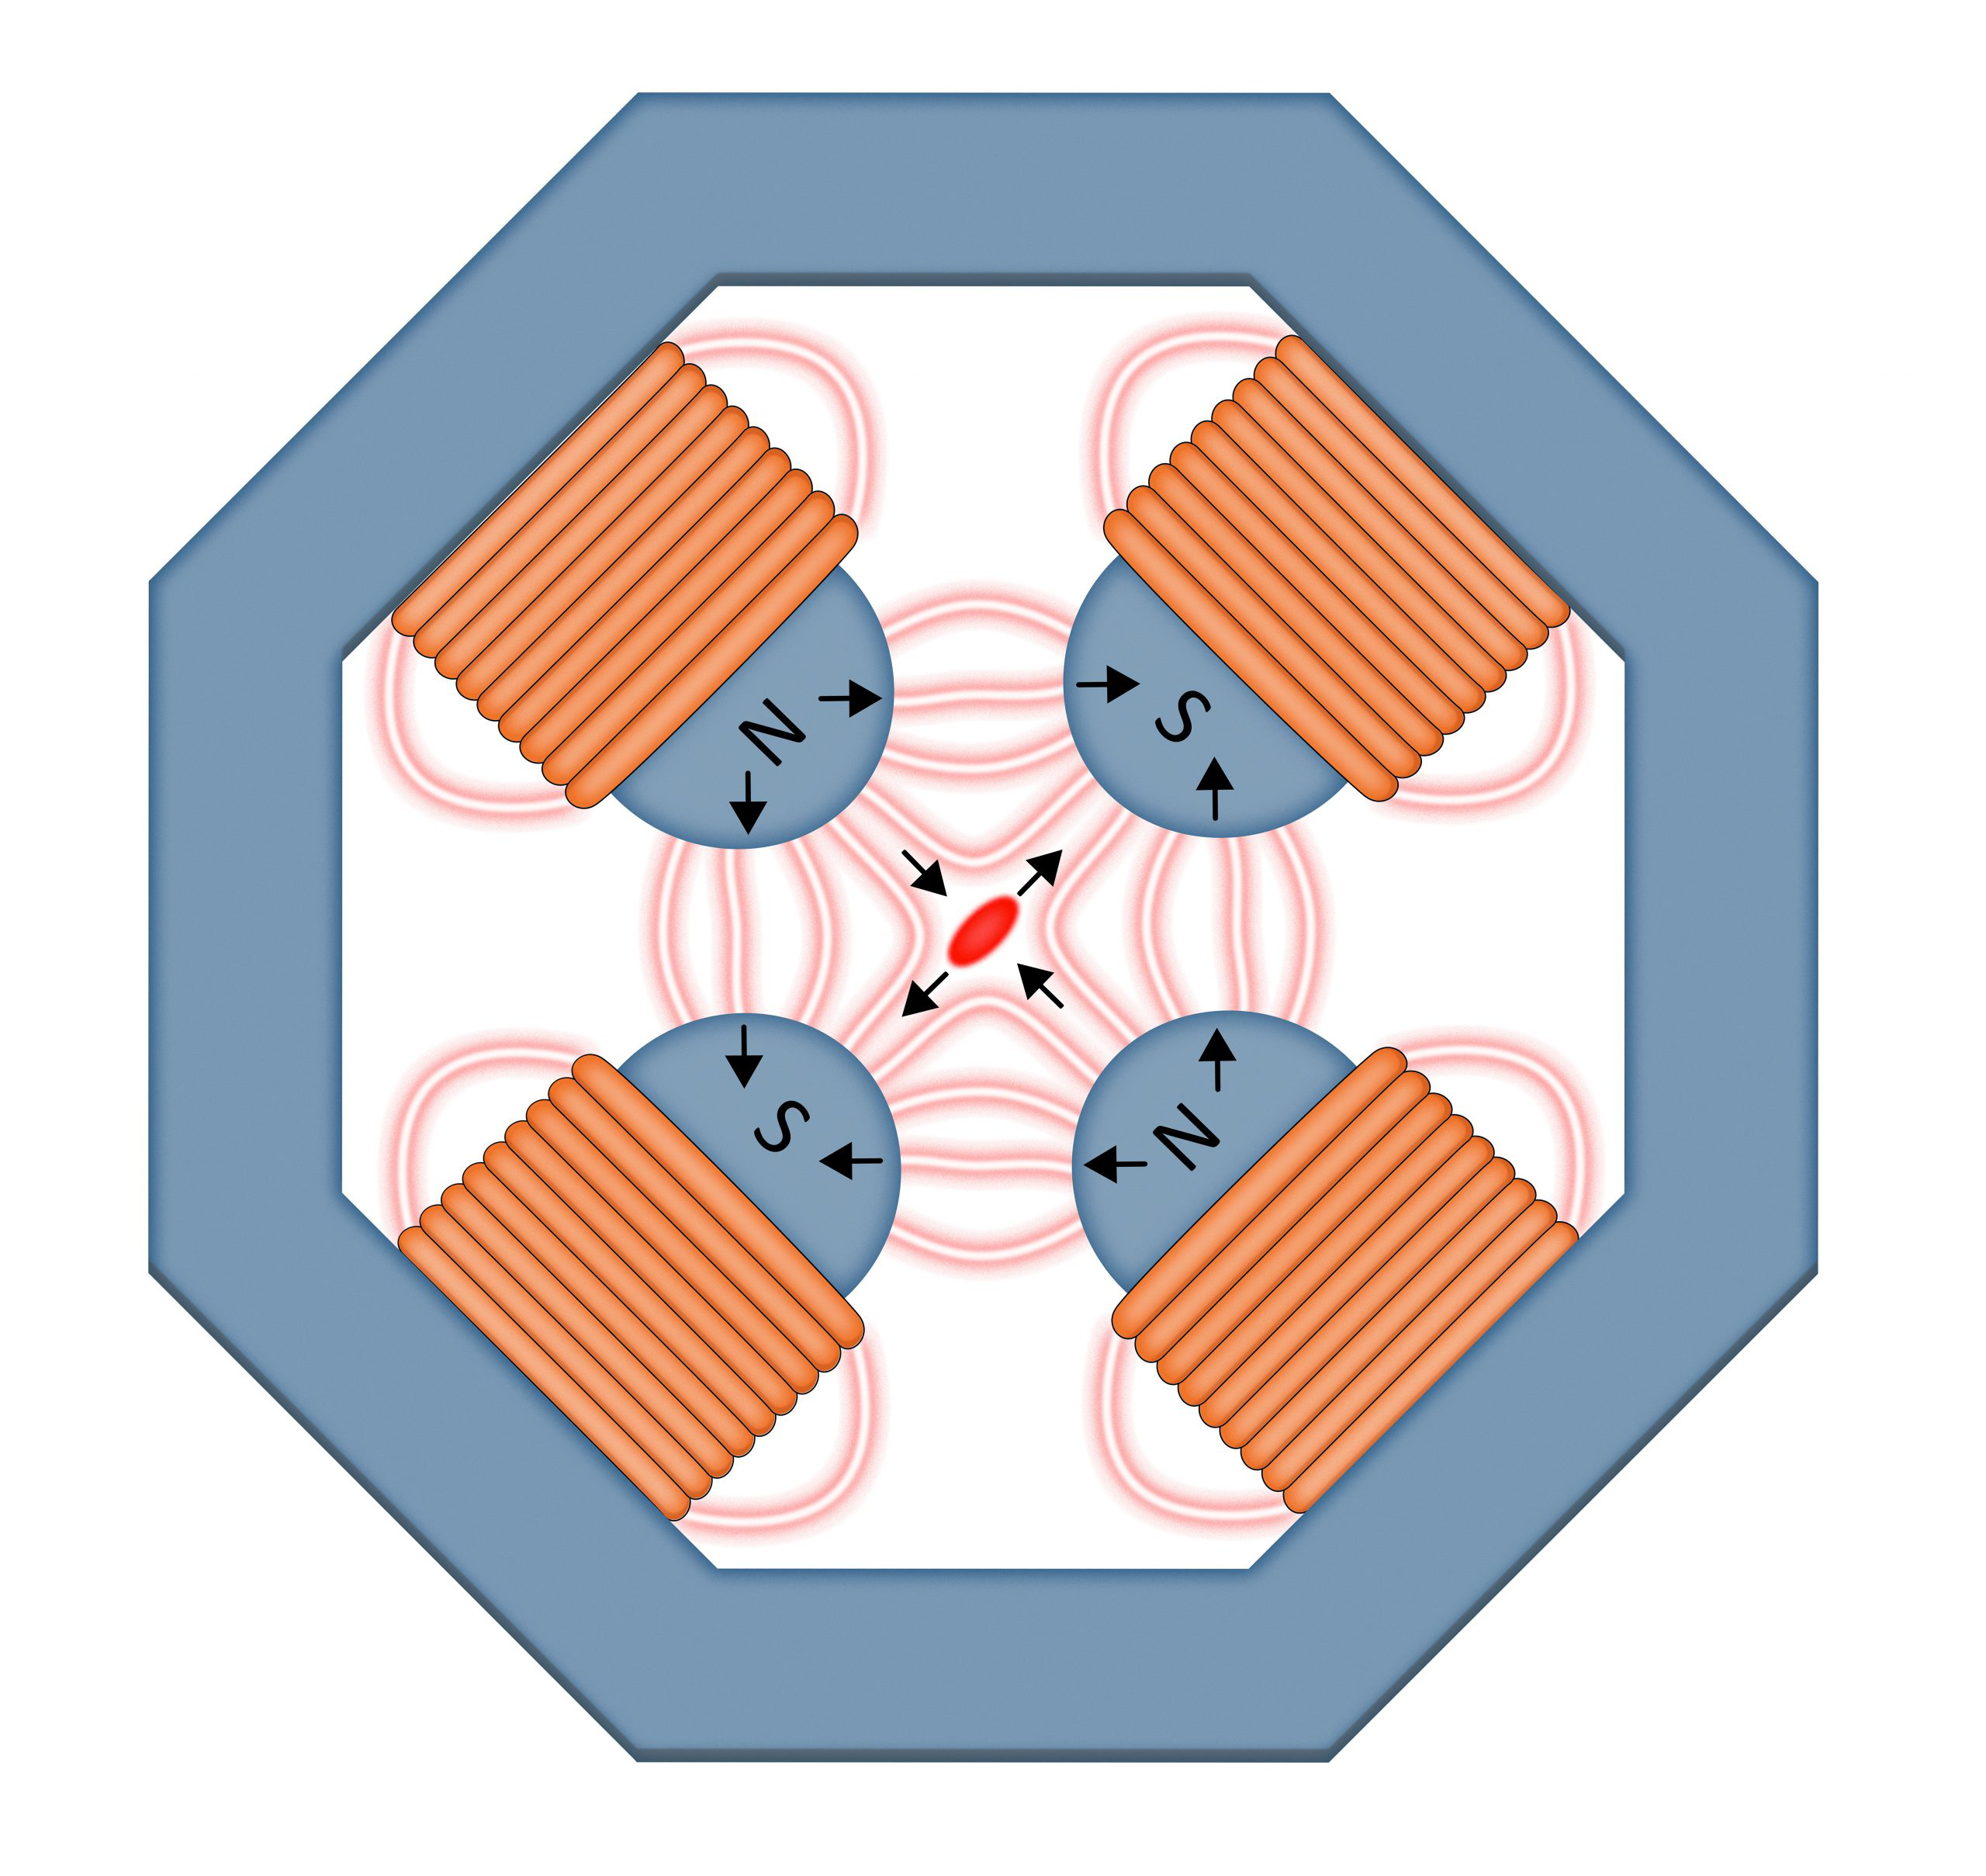
\includegraphics[width=0.9\textwidth]{Problem_4/quadrupoles.png}
    \end{minipage}
    \begin{minipage}{0.45\textwidth}
    \centering
    \scalebox{0.5}{
    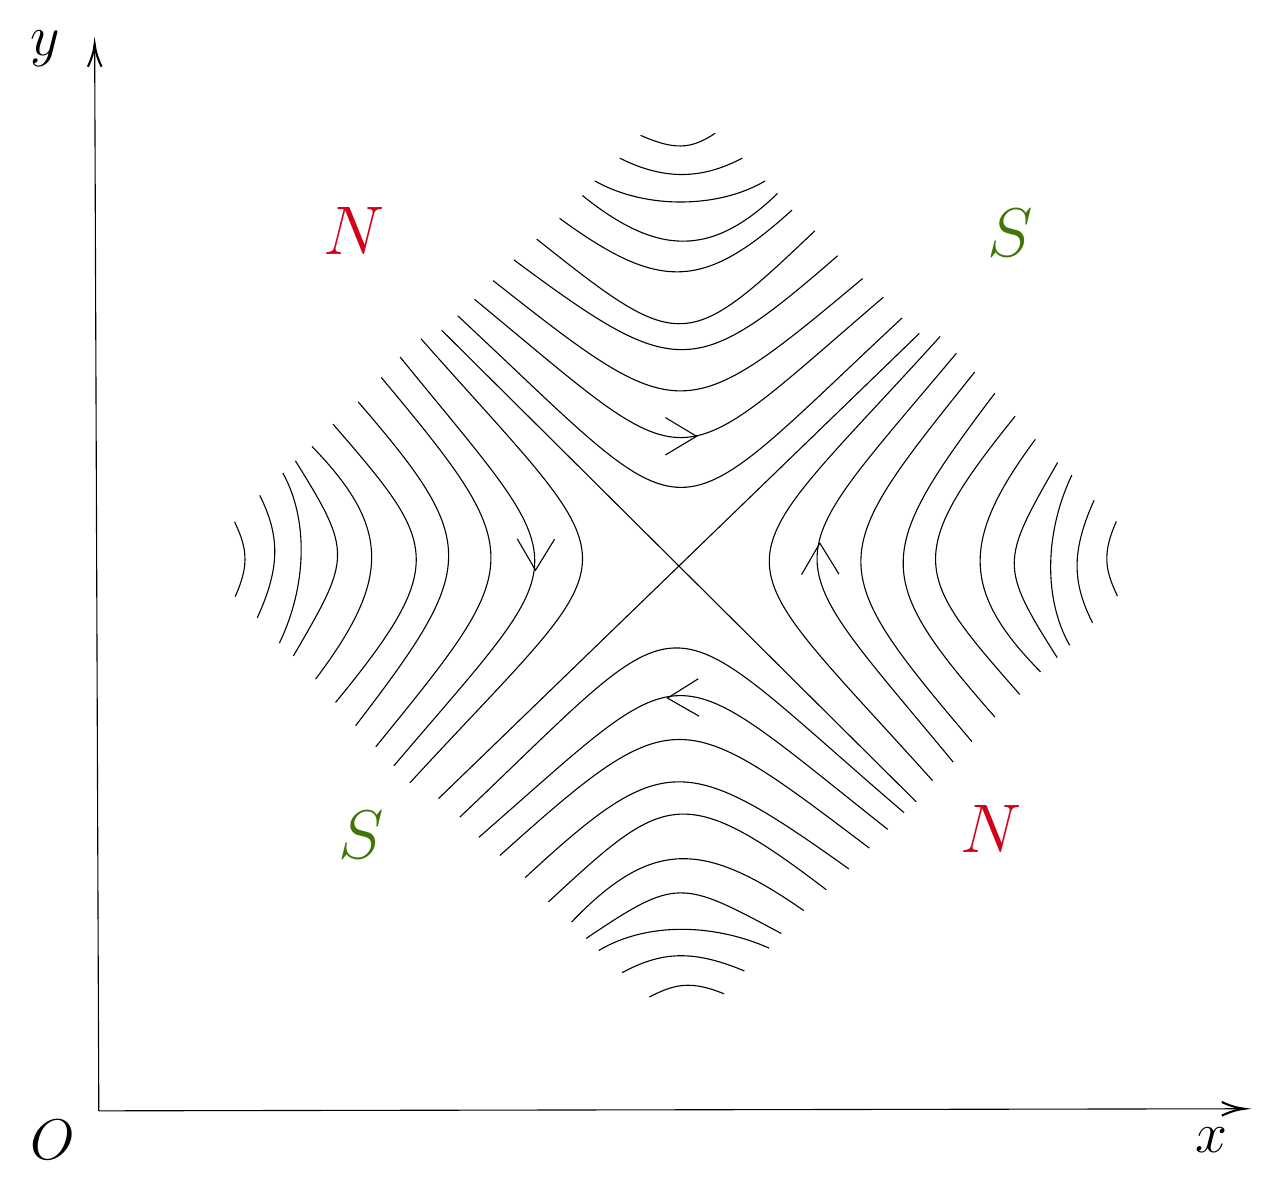
\begin{tikzpicture}[x=0.75pt,y=0.75pt,yscale=-1,xscale=1]
        %uncomment if require: \path (0,642); %set diagram left start at 0, and has height of 642
        
        %Curve Lines [id:da4792522475831378] 
        \draw    (266,156) .. controls (356,227) and (358,227) .. (444,155) ;
        %Curve Lines [id:da18776678628173316] 
        \draw    (257,165) .. controls (365,254) and (349,254) .. (454,164) ;
        %Curve Lines [id:da7579049508332776] 
        \draw    (249,173) .. controls (367,283) and (346,283) .. (463,174) ;
        %Curve Lines [id:da9068961265681277] 
        \draw    (276,146) .. controls (354,204) and (363,204) .. (432,144) ;
        %Curve Lines [id:da6057096352515956] 
        \draw    (287,136) .. controls (356,191) and (359,191) .. (421,132) ;
        %Curve Lines [id:da6124834939512256] 
        \draw    (298,126) .. controls (346,161) and (367,161) .. (410,122) ;
        %Curve Lines [id:da999176140900975] 
        \draw    (309,115) .. controls (345,144) and (371,145) .. (403,114) ;
        %Curve Lines [id:da4412765595880592] 
        \draw    (315,108) .. controls (340,122) and (375,121) .. (397,108) ;
        %Curve Lines [id:da6165862171426286] 
        \draw    (327,97) .. controls (349,108) and (367,107) .. (386,97) ;
        %Curve Lines [id:da5352330674257251] 
        \draw    (337,86) .. controls (353,93) and (361,93) .. (373,85) ;
        %Straight Lines [id:da13696112022895202] 
        \draw    (241.18,179.89) -- (469.82,407.11) ;
        %Straight Lines [id:da612929119766775] 
        \draw    (239.67,405.57) -- (471.33,181.43) ;
        %Curve Lines [id:da9013347475427187] 
        \draw    (209.43,380.62) .. controls (281.45,292.07) and (284.48,289.13) .. (212.07,202.64) ;
        %Curve Lines [id:da8829915710419369] 
        \draw    (218.14,389.8) .. controls (308.32,283.62) and (308,299.62) .. (221.17,192.82) ;
        %Curve Lines [id:da839350917569065] 
        \draw    (225.88,397.96) .. controls (335.11,279.16) and (336.6,303.2) .. (231.24,184.02) ;
        %Curve Lines [id:da09708382750689237] 
        \draw    (199.74,370.42) .. controls (258.67,293.61) and (259.88,282.63) .. (200.95,214.41) ;
        %Curve Lines [id:da6233083389607426] 
        \draw    (190.08,359.22) .. controls (245.86,291.35) and (238.14,282.19) .. (188.87,225.17) ;
        %Curve Lines [id:da9303172125407404] 
        \draw    (180.42,348.02) .. controls (216,300.74) and (217.5,275.76) .. (178.76,235.96) ;
        %Curve Lines [id:da2769813795168756] 
        \draw    (169.77,336.8) .. controls (197.44,289.36) and (198.47,287.38) .. (170.71,242.8) ;
        %Curve Lines [id:da812357712173224] 
        \draw    (162.98,330.66) .. controls (176.4,302.93) and (177.05,270.94) .. (164.65,248.68) ;
        %Curve Lines [id:da730462575275286] 
        \draw    (152.35,318.44) .. controls (163.73,293.67) and (163.05,278.65) .. (153.55,259.45) ;
        %Curve Lines [id:da735579584390504] 
        \draw    (141.68,308.22) .. controls (148.93,292.37) and (147.11,284.33) .. (141.43,272.21) ;
        
        %Curve Lines [id:da9957314369504402] 
        \draw    (447.23,429.41) .. controls (356.24,360.51) and (353.19,357.59) .. (269.26,432.95) ;
        %Curve Lines [id:da42061516499279983] 
        \draw    (456.1,420.39) .. controls (346.85,333.94) and (362.85,333.72) .. (259.14,424.19) ;
        %Curve Lines [id:da6302289013179545] 
        \draw    (463.99,412.36) .. controls (341.47,307.32) and (365.44,305) .. (250,414.44) ;
        %Curve Lines [id:da6314722799353274] 
        \draw    (437.37,439.44) .. controls (358.56,383.22) and (347.55,382.39) .. (281.42,443.65) ;
        %Curve Lines [id:da7627601342878407] 
        \draw    (426.52,449.49) .. controls (356.74,396.1) and (347.86,404.14) .. (292.59,455.36) ;
        %Curve Lines [id:da5517437382717942] 
        \draw    (415.66,459.53) .. controls (367.17,425.61) and (342.16,424.98) .. (303.73,465.09) ;
        %Curve Lines [id:da2523109982366758] 
        \draw    (404.82,470.56) .. controls (356.44,444.56) and (354.42,443.6) .. (310.84,472.9) ;
        %Curve Lines [id:da5531448424788401] 
        \draw    (398.92,477.57) .. controls (370.73,465.12) and (338.74,465.57) .. (316.92,478.74) ;
        %Curve Lines [id:da8274878407169837] 
        \draw    (387.07,488.61) .. controls (361.92,478.1) and (346.93,479.3) .. (328.08,489.46) ;
        %Curve Lines [id:da2516778847803036] 
        \draw    (377.23,499.63) .. controls (361.13,492.94) and (353.16,495.03) .. (341.25,501.14) ;
        
        %Curve Lines [id:da44567985870338966] 
        \draw    (497.97,200.1) .. controls (426.63,289.2) and (423.63,292.16) .. (496.69,378.1) ;
        %Curve Lines [id:da18107514459279583] 
        \draw    (489.19,190.99) .. controls (399.82,297.86) and (400.03,281.86) .. (487.67,387.99) ;
        %Curve Lines [id:da3520275384011575] 
        \draw    (481.38,182.89) .. controls (373.06,302.52) and (371.39,278.5) .. (477.67,396.86) ;
        %Curve Lines [id:da5409134618202889] 
        \draw    (507.73,210.23) .. controls (449.39,287.49) and (448.27,298.48) .. (507.72,366.24) ;
        %Curve Lines [id:da5658457580650191] 
        \draw    (517.48,221.35) .. controls (462.22,289.65) and (470.02,298.75) .. (519.72,355.39) ;
        %Curve Lines [id:da41437201980134053] 
        \draw    (527.22,232.48) .. controls (492.01,280.03) and (490.7,305.02) .. (529.75,344.52) ;
        %Curve Lines [id:da607470080861005] 
        \draw    (537.96,243.62) .. controls (510.65,291.27) and (509.64,293.26) .. (537.75,337.62) ;
        %Curve Lines [id:da3226182027720166] 
        \draw    (544.8,249.7) .. controls (531.59,277.54) and (531.18,309.53) .. (543.76,331.7) ;
        %Curve Lines [id:da59845594322587] 
        \draw    (555.52,261.84) .. controls (544.33,286.7) and (545.13,301.71) .. (554.77,320.84) ;
        %Curve Lines [id:da3781492316292461] 
        \draw    (566.27,271.98) .. controls (559.15,287.89) and (561.02,295.91) .. (566.8,307.99) ;
        
        %Straight Lines [id:da8548346448041899] 
        \draw    (76,556) -- (74.01,44) ;
        \draw [shift={(74,42)}, rotate = 89.78] [color={rgb, 255:red, 0; green, 0; blue, 0 }  ][line width=0.75]    (10.93,-3.29) .. controls (6.95,-1.4) and (3.31,-0.3) .. (0,0) .. controls (3.31,0.3) and (6.95,1.4) .. (10.93,3.29)   ;
        %Straight Lines [id:da8984436400560898] 
        \draw    (76,556) -- (626,555) ;
        \draw [shift={(628,555)}, rotate = 179.9] [color={rgb, 255:red, 0; green, 0; blue, 0 }  ][line width=0.75]    (10.93,-3.29) .. controls (6.95,-1.4) and (3.31,-0.3) .. (0,0) .. controls (3.31,0.3) and (6.95,1.4) .. (10.93,3.29)   ;
        \draw   (349,222) -- (364,231) -- (349,240) ;
        \draw   (295.58,280.6) -- (286.41,295.5) -- (277.59,280.4) ;
        \draw   (365.2,365.83) -- (350,357.16) -- (364.8,347.84) ;
        \draw   (414.6,297.62) -- (423.4,282.5) -- (432.6,297.38) ;
        
        % Text Node
        \draw (183,119.4) node [anchor=north west][inner sep=0.75pt]  [font=\Huge,color={rgb, 255:red, 208; green, 2; blue, 27 }  ,opacity=1 ]  {$N$};
        % Text Node
        \draw (490,407.4) node [anchor=north west][inner sep=0.75pt]  [font=\Huge,color={rgb, 255:red, 208; green, 2; blue, 27 }  ,opacity=1 ]  {$N$};
        % Text Node
        \draw (503,120.4) node [anchor=north west][inner sep=0.75pt]  [font=\Huge,color={rgb, 255:red, 65; green, 117; blue, 5 }  ,opacity=1 ]  {$S$};
        % Text Node
        \draw (190,410.4) node [anchor=north west][inner sep=0.75pt]  [font=\Huge,color={rgb, 255:red, 65; green, 117; blue, 5 }  ,opacity=1 ]  {$S$};
        % Text Node
        \draw (42,559.4) node [anchor=north west][inner sep=0.75pt]  [font=\huge]  {$O$};
        % Text Node
        \draw (603,563) node [anchor=north west][inner sep=0.75pt]  [font=\huge]  {$x$};
        % Text Node
        \draw (42,34.4) node [anchor=north west][inner sep=0.75pt]  [font=\huge]  {$y$};


    \end{tikzpicture}
    }
    \end{minipage} \\
    %\caption{Mô hình tứ cực từ trong thực tế (bên trái) và từ phổ của tứ cực từ (bên phải)}
    \captionof{figure}{Mô hình tứ cực từ trong thực tế (bên trái) và từ phổ của tứ cực từ (bên phải)}
    \label{fig:41}
    \end{center}
    
    Cho từ phổ của một tứ cực từ. Dựa vào hình \ref{fig:41}, hãy xác định phương, chiều của \textbf{đường sức từ} và \textbf{lực điện từ} tác dụng lên một hạt điện tích nhỏ bay vào tứ cực từ với phương vuông góc với trang giấy, chiều ra xa người đọc. 

    \item \textbf{Ứng dụng trong việc hội tụ chùm tia} \\
    Sau khi đã xác định được lực điện từ tác dụng lên hạt điện tích, ta có thể thấy rằng theo phương $y$, hạt sẽ bị đẩy vào bên trong tứ cực từ, còn theo phương $x$, hạt sẽ bị đẩy ra xa tứ cực từ. Hay nói cách khác, nếu ta coi tứ cực từ là một thấu kính thì thấu kính này sẽ \textbf{hội tụ} trên phương $y$ và \textbf{phân kì} trên phương $x$ với cùng một tiêu cự $f$. Nếu ta lật ngược thấu kính đi $90^\circ$ thì thấu kính sẽ phân kỳ trên phương $y$ và hội tụ trên phương $x$.
    
    \begin{figure}[!ht]
    \centering
    \scalebox{0.9}{
    \begin{tikzpicture}[x=0.75pt,y=0.75pt,yscale=-1,xscale=1]
        %uncomment if require: \path (0,424); %set diagram left start at 0, and has height of 424
        
        %Straight Lines [id:da6678677431158608] 
        \draw    (51,378) -- (181,378) ;
        %Straight Lines [id:da673747824550079] 
        \draw    (51,259) -- (181,259) ;
        %Straight Lines [id:da3567165573223894] 
        \draw    (51,259) -- (51,378) ;
        %Straight Lines [id:da4131289268440297] 
        \draw    (181,259) -- (181,378) ;
        %Curve Lines [id:da6284585681017343] 
        \draw    (51,289) .. controls (82,288) and (82,284) .. (83,259) ;
        %Curve Lines [id:da7073873859904605] 
        \draw    (51,346) .. controls (83,348) and (83,348) .. (83,378) ;
        %Curve Lines [id:da3036947661512792] 
        \draw    (149,259) .. controls (150,291) and (150,291) .. (181,291) ;
        %Curve Lines [id:da9150242892043405] 
        \draw    (151,378) .. controls (151,346) and (151,346) .. (182,346) ;
        
        %Straight Lines [id:da8908202829099343] 
        \draw    (245,271) -- (375,271) ;
        %Straight Lines [id:da2173944797906926] 
        \draw    (245,152) -- (375,152) ;
        %Straight Lines [id:da3230976467548934] 
        \draw    (245,152) -- (245,271) ;
        %Straight Lines [id:da37549197915656185] 
        \draw    (375,152) -- (375,271) ;
        %Curve Lines [id:da11844780145514733] 
        \draw    (245,182) .. controls (276,181) and (276,177) .. (277,152) ;
        %Curve Lines [id:da19840673204511416] 
        \draw    (245,239) .. controls (277,241) and (277,241) .. (277,271) ;
        %Curve Lines [id:da07608929271157883] 
        \draw    (343,152) .. controls (344,184) and (344,184) .. (375,184) ;
        %Curve Lines [id:da590005125259021] 
        \draw    (345,271) .. controls (345,239) and (345,239) .. (376,239) ;
        %Straight Lines [id:da8314279294962961] 
        \draw  [dash pattern={on 0.84pt off 2.51pt}]  (181,378) -- (573,162) ;
        %Straight Lines [id:da09601563855642858] 
        \draw    (115,320) -- (205,320) ;
        \draw [shift={(207,320)}, rotate = 180] [color={rgb, 255:red, 0; green, 0; blue, 0 }  ][line width=0.75]    (10.93,-3.29) .. controls (6.95,-1.4) and (3.31,-0.3) .. (0,0) .. controls (3.31,0.3) and (6.95,1.4) .. (10.93,3.29)   ;
        %Straight Lines [id:da8517185652543424] 
        \draw    (115,320) -- (115,228) ;
        \draw [shift={(115,226)}, rotate = 90] [color={rgb, 255:red, 0; green, 0; blue, 0 }  ][line width=0.75]    (10.93,-3.29) .. controls (6.95,-1.4) and (3.31,-0.3) .. (0,0) .. controls (3.31,0.3) and (6.95,1.4) .. (10.93,3.29)   ;
        %Straight Lines [id:da9476216664675472] 
        \draw  [dash pattern={on 4.5pt off 4.5pt}]  (443,162) -- (573,162) ;
        %Straight Lines [id:da7668565905633495] 
        \draw  [dash pattern={on 4.5pt off 4.5pt}]  (443,43) -- (573,43) ;
        %Straight Lines [id:da6517531350813479] 
        \draw  [dash pattern={on 4.5pt off 4.5pt}]  (443,43) -- (443,162) ;
        %Straight Lines [id:da05757003100942071] 
        \draw  [dash pattern={on 4.5pt off 4.5pt}]  (573,43) -- (573,162) ;
        %Straight Lines [id:da1731975813788058] 
        \draw  [dash pattern={on 4.5pt off 4.5pt}]  (38,363) -- (600.25,51.97) ;
        \draw [shift={(602,51)}, rotate = 151.05] [color={rgb, 255:red, 0; green, 0; blue, 0 }  ][line width=0.75]    (10.93,-3.29) .. controls (6.95,-1.4) and (3.31,-0.3) .. (0,0) .. controls (3.31,0.3) and (6.95,1.4) .. (10.93,3.29)   ;
        %Shape: Circle [id:dp49351180655100846] 
        \draw  [fill={rgb, 255:red, 74; green, 144; blue, 226 }  ,fill opacity=1 ] (127,288.5) .. controls (127,287.12) and (128.12,286) .. (129.5,286) .. controls (130.88,286) and (132,287.12) .. (132,288.5) .. controls (132,289.88) and (130.88,291) .. (129.5,291) .. controls (128.12,291) and (127,289.88) .. (127,288.5) -- cycle ;
        %Shape: Circle [id:dp062066057993846346] 
        \draw  [fill={rgb, 255:red, 74; green, 144; blue, 226 }  ,fill opacity=1 ] (291,176.5) .. controls (291,175.12) and (292.12,174) .. (293.5,174) .. controls (294.88,174) and (296,175.12) .. (296,176.5) .. controls (296,177.88) and (294.88,179) .. (293.5,179) .. controls (292.12,179) and (291,177.88) .. (291,176.5) -- cycle ;
        %Straight Lines [id:da517606792137199] 
        \draw    (151,236) -- (130.26,286.65) ;
        \draw [shift={(129.5,288.5)}, rotate = 292.27] [color={rgb, 255:red, 0; green, 0; blue, 0 }  ][line width=0.75]    (10.93,-3.29) .. controls (6.95,-1.4) and (3.31,-0.3) .. (0,0) .. controls (3.31,0.3) and (6.95,1.4) .. (10.93,3.29)   ;
        %Straight Lines [id:da9135691624456295] 
        \draw    (315,124) -- (294.26,174.65) ;
        \draw [shift={(293.5,176.5)}, rotate = 292.27] [color={rgb, 255:red, 0; green, 0; blue, 0 }  ][line width=0.75]    (10.93,-3.29) .. controls (6.95,-1.4) and (3.31,-0.3) .. (0,0) .. controls (3.31,0.3) and (6.95,1.4) .. (10.93,3.29)   ;
        %Shape: Circle [id:dp13300062616731956] 
        \draw  [fill={rgb, 255:red, 74; green, 144; blue, 226 }  ,fill opacity=1 ] (504,104.5) .. controls (504,103.12) and (505.12,102) .. (506.5,102) .. controls (507.88,102) and (509,103.12) .. (509,104.5) .. controls (509,105.88) and (507.88,107) .. (506.5,107) .. controls (505.12,107) and (504,105.88) .. (504,104.5) -- cycle ;
        
        % Text Node
        \draw (57,266.4) node [anchor=north west][inner sep=0.75pt]  [color={rgb, 255:red, 208; green, 2; blue, 27 }  ,opacity=1 ]  {$N$};
        % Text Node
        \draw (158,355.4) node [anchor=north west][inner sep=0.75pt]  [color={rgb, 255:red, 208; green, 2; blue, 27 }  ,opacity=1 ]  {$N$};
        % Text Node
        \draw (160,265.4) node [anchor=north west][inner sep=0.75pt]  [color={rgb, 255:red, 208; green, 2; blue, 27 }  ,opacity=1 ]  {$\textcolor[rgb]{0.25,0.46,0.02}{S}$};
        % Text Node
        \draw (60,355.4) node [anchor=north west][inner sep=0.75pt]  [color={rgb, 255:red, 208; green, 2; blue, 27 }  ,opacity=1 ]  {$\textcolor[rgb]{0.25,0.46,0.02}{S}$};
        % Text Node
        \draw (251,248.4) node [anchor=north west][inner sep=0.75pt]  [color={rgb, 255:red, 208; green, 2; blue, 27 }  ,opacity=1 ]  {$N$};
        % Text Node
        \draw (353,157.4) node [anchor=north west][inner sep=0.75pt]  [color={rgb, 255:red, 208; green, 2; blue, 27 }  ,opacity=1 ]  {$N$};
        % Text Node
        \draw (252,157.4) node [anchor=north west][inner sep=0.75pt]  [color={rgb, 255:red, 208; green, 2; blue, 27 }  ,opacity=1 ]  {$\textcolor[rgb]{0.25,0.46,0.02}{S}$};
        % Text Node
        \draw (355,249.4) node [anchor=north west][inner sep=0.75pt]  [color={rgb, 255:red, 208; green, 2; blue, 27 }  ,opacity=1 ]  {$\textcolor[rgb]{0.25,0.46,0.02}{S}$};
        % Text Node
        \draw (204,297.4) node [anchor=north west][inner sep=0.75pt]    {$x$};
        % Text Node
        \draw (97,218.4) node [anchor=north west][inner sep=0.75pt]    {$y$};
        % Text Node
        \draw (94,298.4) node [anchor=north west][inner sep=0.75pt]    {$O$};
        % Text Node
        \draw (607,38.4) node [anchor=north west][inner sep=0.75pt]    {$z$};
        % Text Node
        \draw (141,211.4) node [anchor=north west][inner sep=0.75pt]    {$A( x_{0} ,y_{0})$};
        % Text Node
        \draw (300,100.4) node [anchor=north west][inner sep=0.75pt]    {$B( x,y)$};
        % Text Node
        \draw (464.5,80.4) node [anchor=north west][inner sep=0.75pt]    {$C( 0,0)$};
        % Text Node
        \draw (286,324.4) node [anchor=north west][inner sep=0.75pt]    {$L$};
        % Text Node
        \draw (466,228.4) node [anchor=north west][inner sep=0.75pt]    {$L$};
        % Text Node
        \draw (23,221.4) node [anchor=north west][inner sep=0.75pt]  [font=\Large]  {$Q_{1}$};
        % Text Node
        \draw (216,116.4) node [anchor=north west][inner sep=0.75pt]  [font=\Large]  {$Q_{2}$};


    \end{tikzpicture}
    } \\
    \caption{Hệ hai thấu kính tứ cực từ}
    \label{fig:42}
    \end{figure}

     Vì tính chất độc đáo này, các nhà khoa học thường dùng các hệ thấu kính tứ cực từ để hội tụ các chùm hạt tích điện trong máy gia tốc hạt. Xét một hệ hai thấu kính tứ cực từ $Q_1$ và $Q_2$ như hình \ref{fig:42}. Các thấu kính cách nhau một đoạn $L$ theo phương $z$, và thấu kính $Q_1$ có tiêu cự trên cả hai phương $x$ và $y$ đều là $f_x = f_y = f$. Ban đầu, có một hạt nhỏ bắn dọc theo phương $z$ vào $Q_1$ tại vị trí $A(x_0, y_0)$. 

    \begin{enumerate}
        \item 
        Xác định tọa độ $B(x,y)$ của hạt khi hạt đến thấu kính $Q_2$ (giả sử các thấu kính đủ rộng để hạt không bị bắn ra ngoài thấu kính).
        \item 
        Tìm điều kiện của $f$ để khi tới điểm cách thấu kính $Q_2$ đoạn $L$, hạt sẽ hội tụ tại điểm $C(0,0)$. Tính tiêu cự $f$ của thấu kính $Q_1$ và $f'$ của thấu kính $Q_2$.
    \end{enumerate}
\end{enumerate}

\begin{flushright}
   \normalcolor(Biên soạn bởi Colevol)
\end{flushright}